\documentclass[10pt]{beamer}
\usepackage[german]{babel}
\usepackage[utf8]{inputenc}
\usepackage{textgreek}
\usepackage{units}


\title[soldering-workshop] % (optional, only for long titles)
{Lötworkshop für Anfänger}
\author{Eileen, towa}
\usetheme{metropolis}

\begin{document}
    \maketitle
    
    \begin{frame}
    \frametitle{Inhalt}
    \begin{itemize}
    	\item{Theorie}
    \end{itemize}
	\end{frame}
    
    \begin{frame}
    \frametitle{Was ist Löten?}
    \begin{itemize}
    	\item{Verbindung zweier Metalloberflächen mit einer Metalllegierung niedrigerer Schmelztemperatur}
    \end{itemize}
	% Bildquellen: https://qph.fs.quoracdn.net/main-qimg-9fcaa4b47839d57b306a2613972ada02.webp
	% https://www.makerspaces.com/how-to-solder/
	\begin{figure}[hbtp]
		\centering
		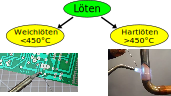
\includegraphics[width=\linewidth*2/3]{images/weich_hartloeten.png}
		\caption{Quelle: ERSA Lötfibel}
	\end{figure}
	\end{frame}

	\begin{frame}
	\frametitle{Elektroniklöten}
	\begin{itemize}
		%TODO: Bilder von Elektronischen Bauteilen und einer Platine
		\item{Verbinden von elektronischen Bauteilen mit einer Platine (PCB)}
		\item{Verwendung von Handlötkolben oder Lötstationen mit \unit[300-400]{$^\circ$C} und \unit[30-80]{W}}
		\item{Als Metallegierung wird Lot oder Lötzinn verwendet}
	\end{itemize}
	\end{frame}

	\begin{frame}
	\frametitle{Das Lot}
	\begin{itemize}
		\item{Metalllegierung aus Zinn, Blei und anderen Metallen}
		\item{Flußmittelseele zur Verbesserung der Flusseigenschaften im Lot enthalten}
		\item{\textcolor{red}{Blei ist ein giftiges Schwermetall! Nicht am Lötplatz essen!}}
	\end{itemize}
	\begin{figure}[hbtp]
		\centering
		\includegraphics[width=\linewidth]{images/lotseele.png}
		\caption{Quelle: ERSA Lötfibel}
	\end{figure}
	\end{frame}

	\begin{frame}
	\frametitle{Was wird benötigt?}
	\begin{itemize}
		\item{Seitenschneider}
		\item{Bausatz}
		\item{Lötkolben}
		\item{Lötzinn}
		\item{Schwamm}
	\end{itemize}
	\end{frame}

	\begin{frame}
	\frametitle{Optionales Zubehör?}
	\begin{itemize}
		\item{Lötstation}
		\item{Heißluftlötkolben}
		\item{Lötpinzette}
		
		\item{Lötdampfabsaugung}
		
		\item{Pinzetten}
		\item{Dritte Hand}
		\item{Lupe}
	\end{itemize}
	\end{frame}

	\begin{frame}
	\frametitle{Lötvorgang}
	\begin{columns}[T] % align columns
		\begin{column}{.33\textwidth}
			\textbf{Benetzen} \newline
			Auf die gereinigte Lötspitze etwas Lot geben.
		\end{column}%
		\hfill%
		\begin{column}{.33\textwidth}
			\textbf{Fließen} \newline
			Die Lötstelle erhitzen und soviel Lot dazu geben wie nötig.
		\end{column}%
		\begin{column}{.33\textwidth}
			\textbf{Binden} \newline
			Erst Lot, dann Spitze von Lötstelle entfernen und anschließen abkühlen lassen.
		\end{column}%
		\hfill%
	\end{columns}
	\end{frame}

	\begin{frame}
	\frametitle{Löten 101}
	\begin{figure}[hbtp]
		\centering
		\includegraphics[width=\linewidth]{images/solder.png}
		\caption{Quelle: Adafruit}
	\end{figure}
	\end{frame}

	\begin{frame}
	\frametitle{Praxisteil: Vorbereitung}
	\begin{itemize}
		\item{Arbeitsplatz überprüfen: Lötkolben, Seitenschneider, Lötzinn, Schwamm, Bausatz vorhanden}
		% TODO: Lötkolben vorheizen evt. am Anfang
		\item{Lötkolben/Lötstation vorheizen (\unit[350]{$^\circ$C})}
		\item{Bausatz auspacken und Teile überprüfen}
	\end{itemize}
	\begin{figure}[hbtp]
		\centering
		\includegraphics[width=\linewidth*5/10]{images/badge.jpg}
		\caption{Der Bausatz}
	\end{figure}
	\end{frame}

	\begin{frame}
		\frametitle{Quellen für Lötzubehör}
		\begin{itemize}
			\item{ELV}
			\item{Watteroth}
			\item{Reichelt}
			\item{Conrad}
		\end{itemize}
	\end{frame}

    
\end{document}
